\documentclass{article}
\usepackage{xeCJK}
\usepackage{fontspec}
\usepackage{ulem}
\usepackage[colorlinks,linkcolor=blue,anchorcolor=blue,citecolor=green,CJKbookmarks=True]{hyperref}
\usepackage{graphicx}
\usepackage{url}
\renewcommand{\normalsize}{\fontsize{12pt}{\baselineskip}\selectfont}
\linespread{1.6}
\begin{document}
\title{国庆水题测试 solution}
\date{\today}
\author{blcup、jiangtao、Wahacer}
\maketitle
\tableofcontents

\newpage
\section{Azur\ Lane}
判断$n$个字符串是否相同.\\
\frame{
\includegraphics[height=50pt]{Image/wuyu.jpg}}\\
直接$stl$真香即可.\\
\sout{帮出题人写题解被D了}\\
\frame{\includegraphics[height=350pt]{Image/a.png}}\\
对于$30\%$的数据,直接$n^2$判断也可以.\\
\newpage
\section{function}
对于$30\%$的数据\\
直接暴力递推,复杂度是$O(TN^2M)$\\
期望得分$30$.\\
\\
对于其中$20\%$的数据\\
即$n$为偶数的情况\\
通过观察找规律,我们发现当$N$为偶数时,$f_{2,1}$就等于$f_{1,n+1}-1$,这个我们可以用矩乘快速幂,快速求得。\\
接下来我们继续观察后面的每一行,发现每一个数都是前一个数$*$2,\\
即  ${\forall i\geq 2,j\geq 2}$  。 $f_{i,j}$=2*$f_{i,j-1}$\\
令$f_{i,1}$=a\\
则$f_{i+1,1}=\sum_{j=1}^Nf_{i,j}=a+2a+...+2^{n-1}*a= (2^n-1)*a$\\
即$f_{i+1,1}=(2^n-1)*f_{i,1}$\\
所以$f_{m,1}=(2^n-1)^{m-2}*f_{2,1}$\\
期望复杂度$O(T(2^3\log{n}+(\log{n}+\log{m})))$
期望得分$20$\\
\\
对于另外$20\%$的数据\\
即$n$为奇数的情况\\
同样通过观察发现当$N$为奇数时,$f_{2,1}=f_{1,n+1}$,同样通过矩乘快速幂,可以快速求得。\\
接下来我们观察后面的每一行,发现任然满足第一列的递推式,但这无法快速求解,我们接着观察发现 \\
当$j$为偶数时$f_{i,j}=f_{i,j-1}*2-1$,当$j$为奇数时$f_{i,j}=f_{i,j-1} *2+1$\\
令$f_{i,1}=a$\\
则$f_{i+1,1}=\sum_{j=1}^Nf_{i,j}=a+(2a-1)+(4a-1)+(8a-3)+(16a-5)+$...\\
对它进行分组求和得 $f_{i+1,1}=(2^n-1)f_{i,1}-f_{1,n-1}$ \\
有了递推式,矩乘快速幂即可。\\
期望复杂度$O(T2^3(\log{n}+\log{m}))$\\
期望得分$20$\\
\\
AC做法1\\
结合奇数和偶数做法即可\\
期望复杂度$O(T(2^3(\log{n}+\log{m})))$\\
期望得分$100$分\\
ps:\\
这道题是去年金哥ACM模拟赛的题,然后他就(懒的出题)拿来给我们考,但当时太弱了,推了一个小时才想出来,最后还打炸了。\\
这道题官方给出的题解是这样的\\
对于任意$i\geq 1$,当$j\geq 3$时,有\frame{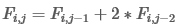
\includegraphics[height=20pt]{Image/1.png}}通过归纳法可以得到\\
得到\\
\frame{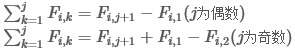
\includegraphics[height=50pt]{Image/2.png}}\\
进而可以推导出\\
\frame{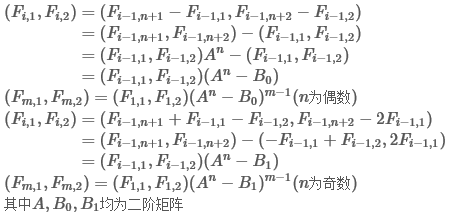
\includegraphics[height=200pt]{Image/3.png}}\\
通过矩阵快速幂求解.\\
哪位大爷能告诉我第一个式子这么推出来的啊QAQ。\\
\\
AC做法2\\
花费了我半个小时,我终于推出来通项公式了。
当$N$为偶数时 \\
$f_{m,1}=\frac{2*(2^n-1)^{m-1}}{3}$\\
当$N$为奇数时
$f_{m,1}=\frac{(2*(2^n-1)^{m-1}+1)}{3}$\\
除法用逆元即可\\
期望复杂度$O(T(\log{n}+\log{m}))$\\
期望得分$100$分\\
证明过程有点长,我就不在这写了,看黑板\\
\newpage
\section{orz}
\sout{orzjtyy}\\
jtyy让我出一道T3,然后发现我的题好像比他的更简单……\\
我们首先来从$orz\ c0per$中清醒过来,考虑一下题面是什么意思.\\
于是我们就得到了一个显而易见的题意\\
给出一个n个点,m条边的DAG,你可以从中选择一些点,被选择的点所能到达的点都无法被选择。 \\
求最多能选出多少点\\
\frame{
\includegraphics[height=50pt]{Image/wuyu.jpg}}\\
有没有觉得这个有点像上课没讲到的东西?\\
像什么DAG最小路径覆盖?\\
要讲DAG最小路径覆盖的话,需要补充两个知识点\\
反链:一个点集,其中任意两点均不可到达。\\
最大(长)反链:反链中点数最多的一条(=最小路径覆盖数)。\\
求法也很简单,由最小路径覆盖数=DAG的点数-最小路径覆盖的边数。\\
把原图的所有节点拆成Xi和Yi,如果DAG中存在边i,j就在二分图中连有向边Xi,Yj,跑二分图匹配。\\
容易得出最大匹配数就是最小路径覆盖的边数,故最小路径覆盖数=DAG的点数-最大匹配数。\\
然后就可以拿到这道题的100分.\\
\\
啊对,至于你说部分分?\\
不知道,或许乱DFS可以拿到很高的分数\\
\sout{谁让这是bzoj的数据呢}\\
\\
那Wahacer不是自爆了么,都没讲还考\\
但请先思考一个问题,DAG最小路径覆盖,和我们所说的最小边覆盖有什么关系?\\
如果在二分图中他们就是一个东西……\\
所以这道题就变成了最小边覆盖,如果你又不慎忘记了最小边覆盖\\
还有一个可以拯救你\\
\textbf{最大独立集}\\
在二分图当中,最大独立集和最小边覆盖相同\\
所以这道题就变得没有自爆!\\
他就是最大独立集,他也是最小边覆盖,他也是DAG最小路径覆盖\\
所以……\\
我们预处理点,如果能相互到达就在二分图当中加边.\\
然后跑最大匹配/最大流/最小割\\
最后答案就是$n-$最大匹配数\\
END.\\
ps:你可能会问我,考试的时候我怎么知道是这样加边呢?\\自己试啊,难不成你要推T2?\\
逃~\\
\end{document}
